We believe that the results presented in this paper are very promising. By applying this preliminary algorithm, we are able to create small patches that the developer can traverse. That being said, additions can be made and parameters can be further refined to optimize the performance of the algorithm in this environment. More importantly, we believe that applying the foundation of our design thinking and methods to new environments could create new socio-technical graphs where spreading activation can provide relevant and small patches like ours.

\section{New Data Types: Text}
Our process can further be extended within the requirements traceability realm by incorporating new node and edge types. In an earlier version of this paper, when talking about unconnected users in Section \ref{unconnectedusers}, we originally said ``at the time the question was asked, the user who will eventually answer the forager's traceability question was not yet connected to the project''. It was only after further reflection that we added ``...by the relationships we chose to express as edges'' to the sentence. In other words, while a user might not have commented or created an issue or been referenced, and therefore is not connected in our current topology, we believe that that user could still be connected in some way. With the addition of new nodes and relationship types, like code and commits, edges between questions and answers, or semantic similarity, unconnected users might be connected, and new and more-insightful relationships might emerge, creating richer and deeper patches.

We'd like to briefly present our preliminary work in semantic similarity, in hopes that it may prove instructive for future work. We decided to extract keywords from bodies of text and to add them as nodes. We drew heavily on PFIS2's approach, visible in Figure \ref{fig:pfis2semantic}, as it had a similar objective of connecting otherwise-unrelated information artifacts with keywords. In order to achieve this scheme, though, we had to extract keywords from comment and issue bodies.

\begin{figure}[ht]
	\centering
	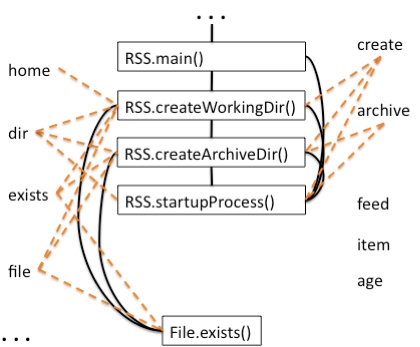
\includegraphics[width=0.5\linewidth]{PFIS2semantic.png}
	\caption{Image From PFIS2 \cite{pfis2} Demonstrating Semantic Similarity Scheme}
	\label{fig:pfis2semantic}
\end{figure}

Extracting keywords in our initial explorations was attempted using two keyword extraction algorithms: TF-IDF ~\cite{tfidf} and RAKE ~\cite{rake}. Briefly, TF-IDF (or Term Frequency--Inverse Document Frequency) is a popular information retrieval metric, applied to a body of documents, which reflects how important a term is in a given document. The most important terms can be treated as keywords. RAKE attempts to extract keywords from a single document by extracting not-commonly-used words or phrases and ranking them relative to each other. Results we observed when implementing both algorithms were similar; we will therefore only mention results from RAKE.

Keywords were only ever part of a shortest path between a question and answer when Degree $\geq$ 3\textemdash perhaps unsurprisingly, the simple ``One or Two Degrees'' cases remain un-touched. In ``Three or Four Degrees'', adding hundreds of keywords provided the algorithm more ways to form shortest paths, but rarely created shorter paths. The average path length before keywords was 2.944, and after was 2.928. Average activation before and after were 0.708 and 0.706, respectively. Min, Max, Median, and Quartiles remained unchanged. Statistically, these differences are insignificant. This suggests that the keywords that we selected added more information, but not necessarily more insightful information. In fact, ``more information'' resulted in a problem: because we were inserting all keywords, networks at the time of question were around 10 times bigger with RAKE keywords, resulting not only in much slower scripting and visulalization performance (we ran out of memory trying to generate graphs for this section), but also larger patches.

\begin{figure}
	\fbox{\parbox{\dimexpr\linewidth-2\fboxsep-2\fboxrule\relax}{\centering Comment 9732 --Issue 4548 -- Person 4 -- Issue 4792 -- Person 691 \\Comment 9732 -- ``workaround'' -- Comment -- Person 691}}\\\\
	\fbox{\parbox{\dimexpr\linewidth-2\fboxsep-2\fboxrule\relax}{\centering Comment 1940 -- Issue 1421 -- Person 196 -- Issue 1432 -- Person 70 \\ Comment 1940 -- ``issue'' -- Comment 2133 -- Person 70}}
	\caption{Two Changed Relationships After Adding Keywords}
	\label{fig:keywords}
\end{figure}

To examine these statistics further, we can look at the two cases where distance was actually shorter: Comment 1940 (from DROOLS) and Comment 9732 (from JBTM), as seen in Figure \ref{fig:keywords}. Before adding keywords, both were four degrees of socio-techincal separation apart. After keywords, they were three. However, in both cases, the shorter path provided through keywords went through generic (to this environment) words: ``workaround'' in the former case and ``issue'' in the latter. This suggests to us that these shorter paths existed by chance, rather than by actual similarlity. If keywords are to be pursued in future work, they should be implemented with far greater discrimination than inserting all RAKE or TF-IDF keywords, and they should be studied most intensely in distant cases where otherwise they would be four or more degrees of socio-technical separation apart. 

\section{Systematic Spreading Activation Parameters}
Future work could also be conducted on the implementation of the algorithm itself. Our decay, frequency reward, weights, and patch cutoff parameters were set through observation and trial and error. More sophisticated statistical analyses, like machine learning algorithms, could help better set these parameters. Our method only suggested the first patch for foraging; in reality, a forager will go through several patches in search of their prey. To accommodate this pattern, this work could be extended to multiple-patch creation. Already, we have begun exploring ways to remove the need to manually determine weight for each type of relationship, and considered a possible approach to implement frequency incentives.

\subsection{Weight}
When establishing weights for our algorithm, our objective was to have activation flow towards people and information artifacts that presented knowledge on the initially-activated points. We achieved this by allowing activation to flow more freely towards users who likely had authority on a given comment or issue. This approach does require us, however, to come up with a new weight for each new relationship added. It would be beneficial, therefore, to have the same properties emerge from an automated process.

While there could be many approaches for future work in this direction, we would like to present one promising direction that arose in our research. With the objective of spreading activation towards knowledge, and with the postulate that knowledge is typically centered around the issue where the comment is posted, we removed weights, and activated the issue in addition to the comment. We then spread activation (with a higher decay of 0.25 rather than 0.1). In other words, as a replacement to weighting schemes, we started the spreading of activation from comment \textit{and issue}. Remarkably, this had similar results in some initially-explored metrics. Furthermore, if we only activated the issue or only increased decay, our results weren't as successful. A brief summary of these results can be seen in Table \ref{tab:weightless}. The graphs in Appendix \ref{app:cytoscape} were actually generated during this test. The activation-cutoff graph was the same both in the Weighting scheme and the Weightless + Activated Issue scheme.

\begin{table}[ht]
	\caption{Activating Comment \textit{and} Issue Instead of Weighting Edges}
	\centering
	\begin{tabular}{ |c||c|c|c|c|  }
		\hline
		& \makecell{ Median Patch \\ Size A $\geq$ 0.45} & \makecell{ Median Patch \\ Size A $\geq$ 0.72} & \makecell{ \% Answers in \\ Patch A $\geq$ 0.45} & \makecell{ \% Answers in \\ Patch A $\geq$ 0.72} \\
		\hline
		\makecell{Weighting \\ Edges} & 286 & 5 & 100 & 84.8 \\
		\makecell{ Weightless + \\ Activate Issue} & 204 & 6 & 96.8 & 84.8 \\
		\hline
		Only Weightless & 192 & 3 & 84.8 & 24.0 \\
		\hline
	\end{tabular}
	\label{tab:weightless}
\end{table}

Table \ref{tab:weightless} shows that both weightless schemes have slightly smaller patches, which makes sense considering the more aggressive decay. Also, it shows that only with the issue activated does performance (as measured by answers in patches) come close to the weighted method explored earlier in this paper.

\subsection{Frequency Incentives}
We think that incentivizing frequency is an important aspect of our algorithm; a person who comments on an issue multiple times should have higher activation than one with only one comment. However, our approach of giving a bonus to nodes that were frequently visited by our traversal was not extremely effective. It was hard to find a value that would provide that incentive while still allowing activation to decay.

One method we suspect might prove successful is counting number of shortest paths. Consider our three frequency examples, in Figures \ref{fig:3degCollab}, \ref{fig:3degContrib}, and \ref{fig:4degContrib}. The shortest path between the answer node and the question node is three or four degrees, but there were multiple ways that this distance could be achieved. We see this as being the same as the frequency we want to incentivize. Of course, as distance increases, number of shortest paths increases, so any metric developed to incentivize frequency through number of shortest paths should be inversely proportional to distance, as well. Finally, in initial tests using NetworkX, counting number of shortest paths was extraordinarily slow, increasing runtime by a factor of 10 or more.

\section{New Domains}
Most importantly, this method could be extended to other socio-technical tasks. We believe that applying the foundation of our design thinking and methods to new domains could create socio-technical graphs where spreading activation can provide relevant and small patches like ours. We see these domains as being anything from suggesting movies based on the cast and crew that link them together, to gathering evidence of work on requirements for safety certification.

\begin{figure}[ht]
	\centering
	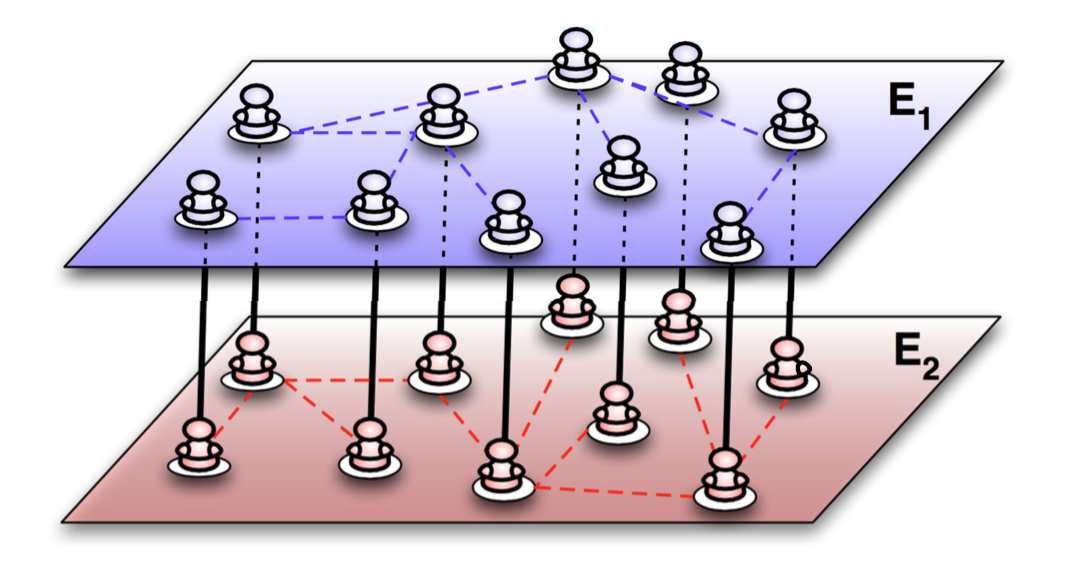
\includegraphics[width=0.5\linewidth]{composite.png}
	\caption{A Composite Network with Two Sets of Nodes $E_{1}$ and $E_{2}$ Source: ~\cite{memescomposite}}
	\label{fig:composite}
\end{figure}

One particular domain that has caught our attention is that of composite networks. A composite network could be defined as a graph with one set of nodes and two or more distinct sets of edges, like in Figure \ref{fig:composite}. Wei et al. explored composite networks when using epidemic models to analyze how memes might spread over two social networks that share the same set of users (e.g. people who have both a Facebook and Twitter account) ~\cite{memescomposite}. We think that similar network topologies would be very interesting to explore with spreading activation.

Immediately, multi-Jira-project analysis comes to mind. Users who participate in multiple projects, or shared code-bases across projects, would serve as our composite nodes; each project's issues and comments would provide a distinct set of edges. Connections from one project would provide a set of deeper context to another.

Reaching further, spreading activation in composite networks could be applied to everyday Internet life. In a world where algorithms provide us only with news we want to read, and we follow friends and influencers who say only what we are already thinking, polarization is driving a wedge into modern-day society. We imagine an application of our spreading activation algorithm that builds patches of content relevant to an issue, not in an issue tracker, but in our society, by spreading activation over the people and news stories across multiple composite networks.
